\section{Entity Relationship Diagram}
\subsection{Entities}
We will have seven entities: user, post, comment, topic, question, Q\&A post, and answer.

A user is any individual writing a post on Ask Us. The user entity will have five attributes: ID, name, email, password, and points. ID will be the primary key. Points is a metric of rating.

Topic is a way a user can categorize his quesion thus getting better targeted responses. A user can also follow a topic of interest. The topic entity will have three attributes: ID, name, and description. ID will be the primary key.

A post is anything a user writes. That can either a quesion, an answer, or a comment. The post entity wil have four attributes: ID, body, date-time, and points. ID will be the primary key.

A comment what a user would write if was to comment on a post. The comment entity is special type of Post. Comment itself has no attributes.

A Q\&A post is either a question or an answer that a user posts. The Q\&A post entity has no attributes of its own.

A question is what a user would post if he wanted to receive a solution to his inquiry. The question entity has one attribute called title.

An answer is what a user would post if he wanted to give a solution to a inquiry. The answer entity has one attribute called accepted.

\subsection{Relations}
The user entity has a relation with the topic enitity, called follows. In the follows relation, there can be many topics a user can follow but it is not mandatory for a user to follow any topic. In the same light, there can be topics followed by no one or by one or many users.

The user entity also has a relation with the post enitity, called wrote. In the wrote relation, the user can write anywhere from many to no posts. A post can only be written by exactly one user.

The comment enitity has two relations with the post enitity. One relation is called belongs to. In the belongs to relation, a post can have no or one or many comments. In this relation, a comment can only be a comment on exactly one post. The other relation is called is a. In the is a relation, a particular comment is related to exactly one post. In this relation, a post does not neccessarily have to be related to a comment, but if it is, it is related to exactly one comment.



\subsection{Diagram}

Figure \ref{erd} shows the entity relationship diagram for the database we are to make for Ask Us.

\begin{figure}[htb]
	\centering
	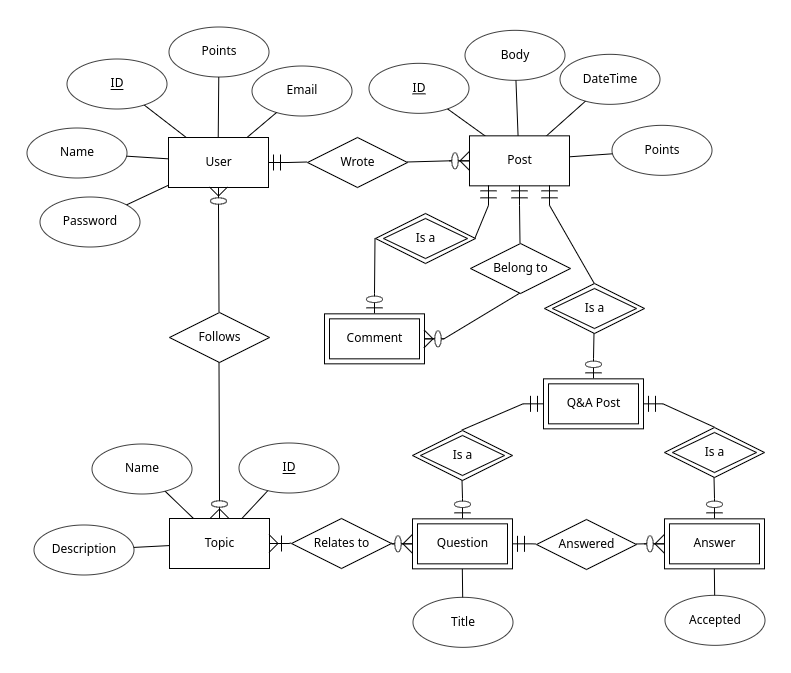
\includegraphics[width=\linewidth]{../ERD/erd.png}
	\caption{An ERD for the database for Ask Us}
	\label{erd}
\end{figure}
